% =======================================================================
% =                                                                     =
% =======================================================================
% -----------------------------------------------------------------------
% - Author:     Chaua Queirolo                                          -
% - Version:    001                                                     -
% -----------------------------------------------------------------------
\documentclass[a4paper,11pt]{article}    

% =======================================================================
% PACKAGES
% =======================================================================

% Language support
\usepackage[brazil]{babel}
\usepackage[utf8]{inputenc}
\usepackage[T1]{fontenc}
\usepackage{ae,aecompl}

% Configuration
\usepackage{url}
\usepackage{enumerate}
\usepackage{color}
\usepackage[svgnames,table]{xcolor}
\usepackage[margin=2cm,includefoot]{geometry}

% Tabular
\usepackage{multirow}
\usepackage{multicol}

% Images
\usepackage{graphicx}
\usepackage{caption}
\usepackage[scriptsize]{subfigure}
\usepackage{epstopdf}
\usepackage{float}% http://ctan.org/pkg/{multicol,lipsum,graphicx,float}

% Math
\usepackage{mdwtab}	% bug rowcolor
\usepackage{amssymb}
\usepackage{amsmath}
\usepackage{footnote}

% References
\usepackage[sort,nocompress]{cite}

% =======================================================================
% VARIABLES
% =======================================================================

% Space between the lines in a table
\renewcommand{\arraystretch}{1.3}

% Define a new column type
\newcolumntype{x}[1]{>{\raggedright\hspace{0pt}}p{#1}}%

% Controle das Margens
\sloppy
\tolerance=9999999

% Espaço entre colunas
\setlength{\columnsep}{.9cm}


% Configuration
\usepackage{lipsum}
\usepackage{blindtext}

% =======================================================================
% HEADER
% =======================================================================

\title{Algoritmos Genéticos}
\author{Felipe Eduardo Lopes\\E-mail: {\tt felipe\_lopes@outlook.com}}
\date{}

\newenvironment{Figure}
  {\par\medskip\noindent\minipage{\linewidth}}
    {\endminipage\par\medskip}

% =======================================================================
% DOCUMENT
% =======================================================================
\begin{document}

\maketitle

\begin{multicols}{2}

\section{Introdução}
Algoritmo Genético é uma técnica de IA, foi criada com o objetivo de limitar determinados processos observados na evolução natural das espécies. As técnicas consistem em solucionar problemas do mundo real de forma otimizada, sendo aplicável em diversas áreas. \cite{ref:ref_01}

\section{Descrição do algoritmo genético e estratégias evolutivas}
- O algoritmo genético funciona da seguinte maneira.
Inicialmente é gerada uma população formada por um conjunto aleatório de indivíduos, que podem ser vistos como possíveis soluções para o problema.\\
- Durante o processo evolutivo, a população é avaliada, sendo que para cada indivíduo é atribuído uma nota, normalmente chamado de fitness, que reflete sua habilidade de adaptação a determinado ambiente.\\
- Uma porcentagem dos indivíduos é mantido, essa seleção é feito por um dos métodos existentes.\\
- Os membros mantidos pela seleção podem sofrer mutações em suas características fundamentais por meio de cruzamentos (crossover),  gerando descendentes para a próxima geração.\\
- Esse, processo, chamado de reprodução, é repetido até uma solução satisfatória seja encontrada, ou até que o número de gerações sejam alcançados.\\

\subsection{Inicialização}
Os cromossomos de uma população devem ser gerados de forma aleatória. O objetivo é aumentar a diversidade genética da população, caso a inicialização da população não seja feita de forma aleatória, esta poderá convergir prematuramente, ou seja, em um curto espaço de  tempo a população terá indivíduos muito semelhantes entre si.\\
Após a criação da população inicial, é necessário avaliar todos os cromossomos gerados (fitness).

\subsection{Avaliação do fitness}
O cálculo do fitness é o único elo entre o algoritmo genético e o problema proposto, é a única parte não genética do algoritmo e deve ser capaz de identificar todas as restrições e objetivos, ou seja, a função de aptidão deve ser específica para cada problema.É nessa função que a definição do problema é realizada.
 
\subsection{Seleção}
A seleção é realizado logo após o cálculo fo fitness. Sua implementação é baseada no processo de seleção natural, onde os indivíduos mais capazes possuem maior probabilidade de gerar descendentes, em quanto os menos capazes, dependendo da técnica de seleção utilizada também pode realizar descendentes, porém com probabilidade menor.\\
Existem diversas técnicas para realizar a seleção dos indivíduos, uma das mais famosas é a seleção pela Roleta Viciada e a seleção por torneio.

\subsubsection{Roleta Viciada}
Nessa técnica, a seleção dos cromossomos ocorre de forma proporcional ao seu valor de fitness, sendo que os cromossomos de uma população são representados em uma roleta, onde ocupam um espaço proporcional ao seu valor de fitness. Os cromossomos que possuírem um valor de fitness alto terão um espaço maior na roleta, aumentando sua probabilidade de ser escolhido, já com valor de fitness menor, a probabilidade de ser escolhido é muito menor, pois seu espaço na roleta será menor. Nessa técnicas os piores indivíduos tem uma baixa probabilidade de gerar descendentes. Na figura 1 é possível ver um exemplo da roleta viciada.

\begin{Figure}
	\centering 
	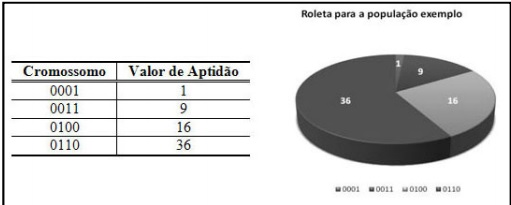
\includegraphics[width=8cm, height=4cm]{figura1}
	\captionof{figure}[]{Exemplo roleta viciada. Fonte: Thatiane de Oliveira Rosa, Hellen Souza Luz}
	\label{medium}
\end{Figure}

\subsubsection{Torneio}
Essa técnica se dá a partir da escolha de n cromossomos na população atual, de forma aleatória. Dentre tais cromossomos escolhidos, o com maior valor de fitness é selecionado para compor a população intermediária. Em seguida, os demais cromossomos são recolocados na população e realiza-se o mesmo processo até que a população intermediária esteja completa. Nessa técnica os piores indivíduos não tem chance de gerar descendentes.

\subsection{Crossover}
O processo de cruzamento é utilizado após a realização da seleção. Nessa fase, ocorre a troca de segmentos entre pares de cromossomos selecionados para originar novos indivíduos. A ideia é propagar as características positivas dos indivíduos para seus descendentes.\\
As técnicas mais comuns de crossover é com um e dois cortes.\\

\subsubsection{Crossover com um ponto de corte}
No método de corte único, é escolhido um ponto de corte aleatório e a partir desse ponto o material genético dos pais é trocado dando origem a dois novos cromossomos, formados pela combinação das características genéticas dos pais. Na figura 2 podemos observar o comportamento dessa técnica.
\begin{Figure}
	\centering 
	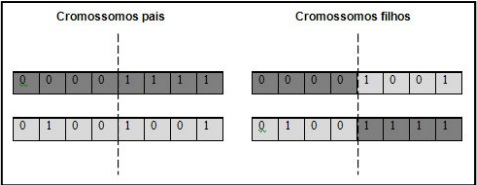
\includegraphics[width=8cm, height=4cm]{figura2}
	\captionof{figure}[]{Crossover com 1 ponto de corte. Fonte: Thatiane de Oliveira Rosa, Hellen Souza Luz}
	\label{medium}
\end{Figure}

\subsection{Crossover com dois pontos de corte}
No método de dois cortes, é escolhido dois pontos de corte aleatoriamente. A partir desses pontos os matérias dos pais são trocados de forma intercalada, como podemos observar na figura 3.
\begin{Figure}
	\centering 
	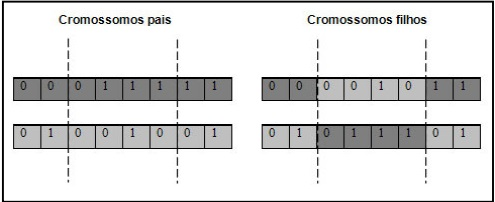
\includegraphics[width=8cm, height=4cm]{figura3}
	\captionof{figure}[]{Crossover com 2 pontos de corte. Fonte: Thatiane de Oliveira Rosa, Hellen Souza Luz}
	\label{medium}
\end{Figure}

\subsection{Mutação}
Mutação é realizada logo após o crossover e tem como objetivo realizar modificações em determinadas propriedades genéticas de uma população. É importante uma vez que possibilita à população atual obter novas propriedades. Essa fase é indispensável, já que permite a introdução e manutenção da diversidade da população. Uma porcentagem de mutação deve ser informado nessa técnica que determinará o volume de indivíduos que sofrem mutação da população.

\subsection{Atualização}
Na atualização a população antiga é substituída pela nova população, formada pelo crossover dos indivíduos selecionados da população anterior. As formas mais conhecidas de atualização são (x+y) e (x,y). Na primeira estratégia, chamada também de soma a população anterior convive com a nova população. Já a segunda estratégia, também conhecida como eletismo e geralmente uma porcentagem muito pequena é selecionada para a próxima geração, pois corre risco de convergência prematura.

\section{Exemplos de aplicações}
\subsubsection{Telecomunicações}
Segundo Blanchard (1994), no WCCI'94 – World Congress on
Computational Intelligence – ocorrido em Orlando, na Flórida, mostrou uma série de soluções promissoras a situações reais utilizando Algoritmos Genéticos. Blanchard mostrou o caso da US West, uma companhia regional de telecomunicações do estado do Colorado, que vem usando um sistema baseado em AGs que possibilita projetar, em duas horas, redes óticas especializadas, trabalho que levaria seis meses utilizando especialistas humanos. O sistema produz resultados ainda 10% (dez por cento) melhores
que os realizados pelo homem. A companhia estimava, naquele momento, que o sistema possibilitará uma economia de 100 milhões de dólares até o final do século. \cite{ref:ref_02}

\subsubsection{Música}
Foi apresentado em 1999 na CEC99 – IEEE – International Conference on Evolutionary Computation um ambiente interativo, utilizando Algoritmos
Genéticos, para a avaliação de músicas (seqüências de acordes) tocadas em arquivos MIDI. No caso, os indivíduos da população foram definidos em grupos
de quatro vozes (soprano, contralto, tenor e baixo) ou coros. Cada um é avaliado segundo três critérios: melodia, harmonia e oitavas. A composição
destes três critérios definia a aptidão (fitness) definida pela função de seleção, que retorna o melhor indivíduo ou melhor coro. Um ciclo genético é
operacionalizado, criando novos indivíduos dos anteriores e procurando sempre pelo melhor. Quando um novo grupo é selecionado, ele é tocado em
MIDI. A duração do ciclo genético determina o ritmo da evolução. O sistema criado foi denominado Vox Populi. (FUKUSHIMA, 1999).
\cite{ref:ref_02}

\subsubsection{Matemática}
Utilizado para resolver vários problemas matemáticos e probabilísticos, desde os mais simples até os mais complexos. Por exemplo encontrar os zeros de uma função.

\section{Conclusão}
Através das técnicas apresentas é possível realizar a implementação de uma rede e simular várias operações genéricas da mesma forma como estas se dão na natureza.

\bibliographystyle{plain}
\bibliography{referencias}

\end{multicols}
\end{document}

